ATLAS high-mass Drell--Yan 7 TeV~\cite{Aad:2013iua} 

ATLAS low-mass Drell-Yan 7 TeV~\cite{Aad:2014qja}

ATLAS Z PT 7 TeV~\cite{Aad:2014xaa}

ATLAS Z phistar 7 TeV~\cite{Aad:2012wfa}

CMS Drell--Yan 7 TeV~\cite{Chatrchyan:2013tia}

CMS Drell--Yan 8 TeV~\cite{CMS:2014jea}

CMS angular coefficients 8 TeV~\cite{Khachatryan:2015paa}

CMS Z PT and rapidity 8 TeV~\cite{Khachatryan:2015oaa}

\begin{figure}[p]
    \centering
    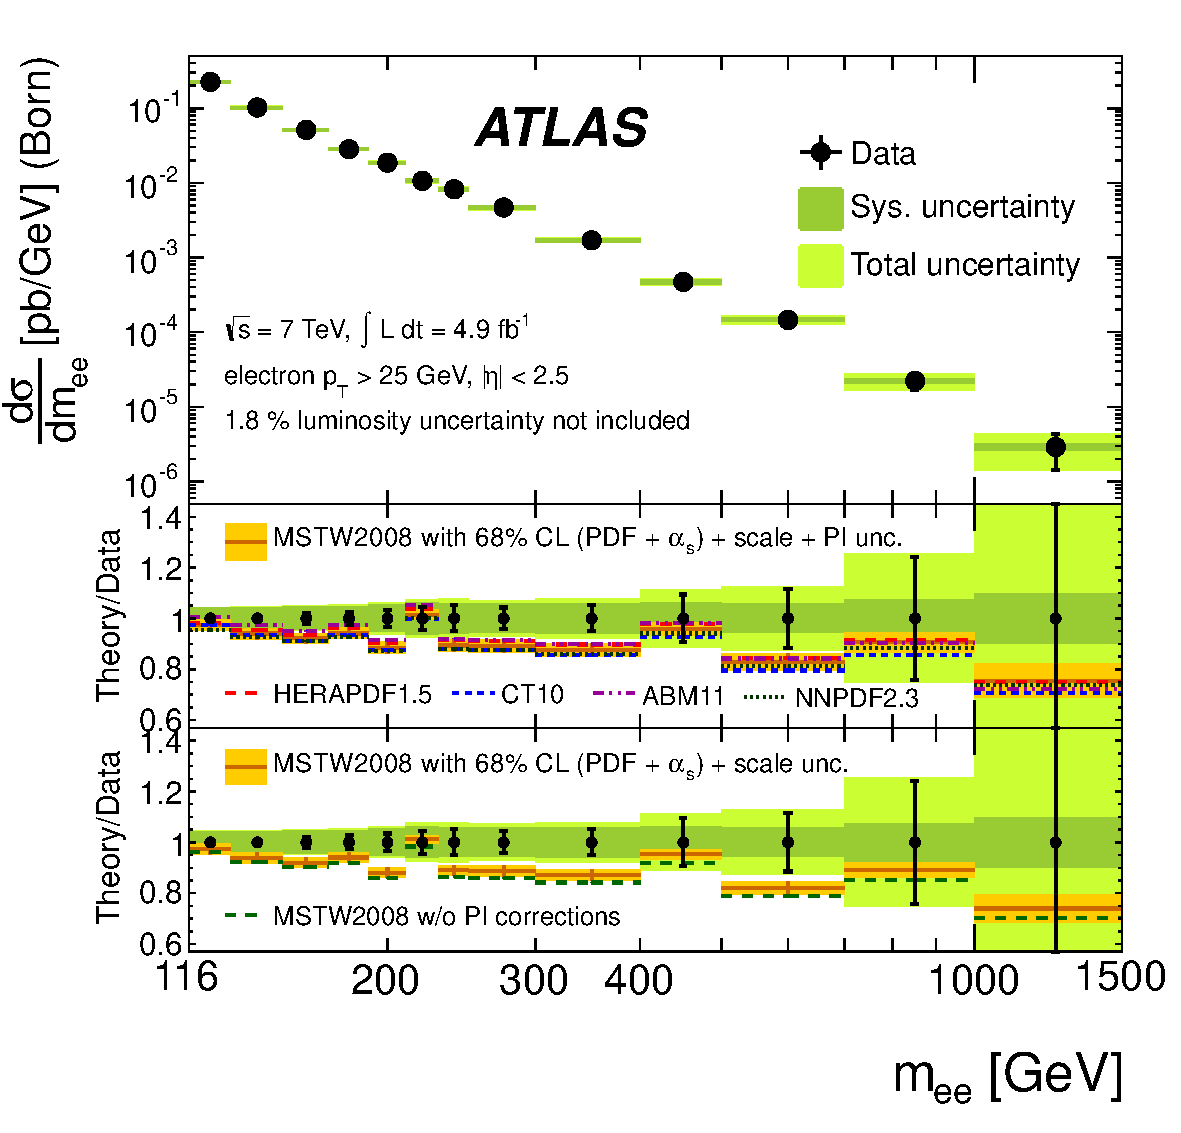
\includegraphics[height=0.3\textheight]{figures/sss-inclboson-drellyan-atlas7tev}
    \caption{Measured differential cross-section at the Born level within the fiducial region (electron $p_T > 25$ GeV and $|\eta| < 2.5$) with statistical, systematic, and combined statistical and systematic (total) uncertainties, excluding the 1.8\% uncertainty on the luminosity. The measurement is compared to FEWZ 3.1 calculations at NNLO QCD with NLO electroweak corrections using the $G_{\mu}$ electroweak parameter scheme. The predictions include an additional small correction from single-boson production in which the final-state charged lepton radiates a real W or Z boson. On the left, in the upper ratio plot, the photon-induced (PI) corrections have been added to the predictions obtained from the MSTW2008, HERAPDF1.5, CT10, ABM11 and NNPDF2.3 NNLO PDFs, and for the MSTW2008 prediction the total uncertainty band arising from the PDF, $\alpha_s$, renormalisation and factorisation scale, and photon-induced uncertainties is drawn. The lower ratio plot shows the influence of the photon-induced corrections on the MSTW2008 prediction, the uncertainty band including only the PDF, $\alpha_s$ and scale uncertainties. On the right, the results are shown for a restricted range of $m_{ee}$.}
    \label{fig:sss-inclboson-drellyan-atlas7tev}
\end{figure}

\begin{figure}[p]
    \centering
    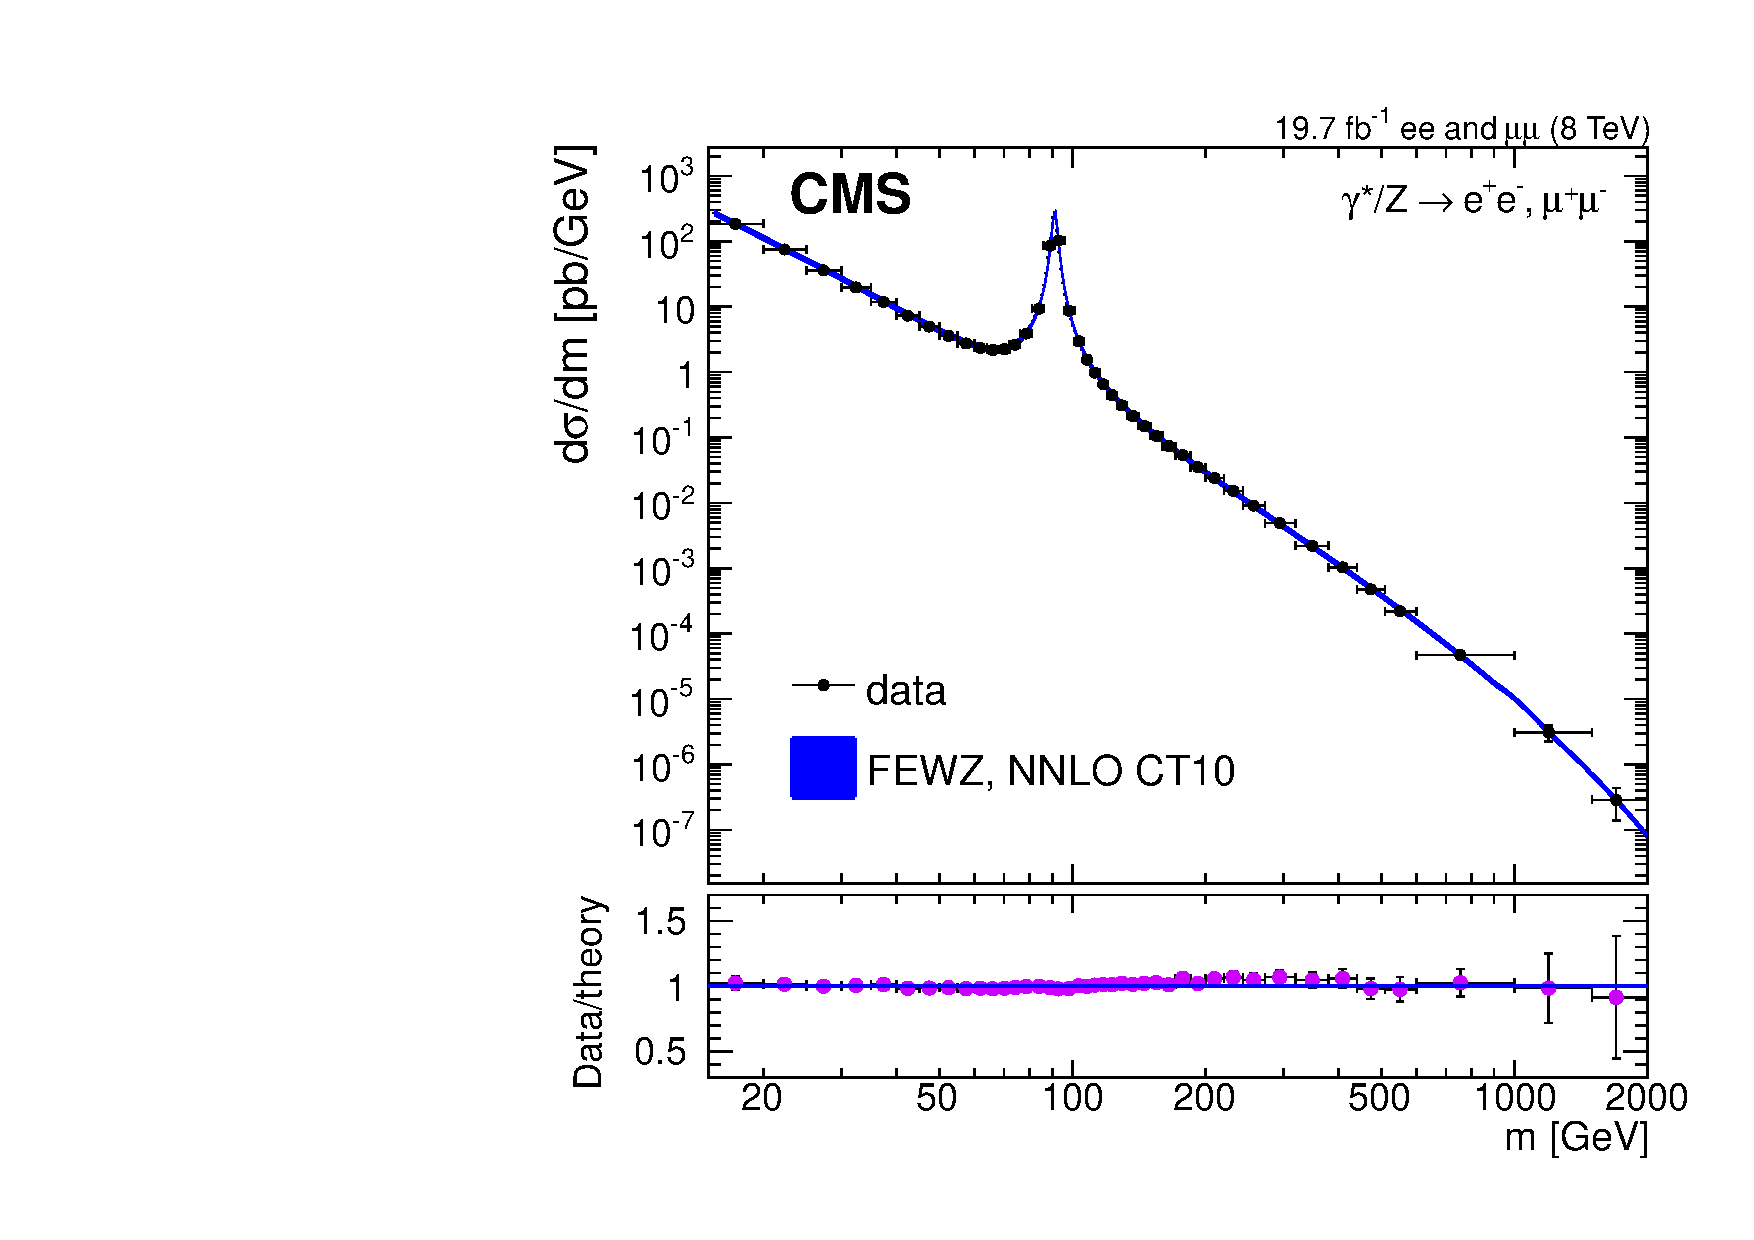
\includegraphics[height=0.3\textheight]{figures/sss-inclboson-drellyan-cms8tev}
    \caption{}
    \label{fig:sss-inclboson-drellyan-cms8tev}
\end{figure}

